\documentclass[twoside]{book}

% Packages required by doxygen
\usepackage{fixltx2e}
\usepackage{calc}
\usepackage{doxygen}
\usepackage[export]{adjustbox} % also loads graphicx
\usepackage{graphicx}
\usepackage[utf8]{inputenc}
\usepackage{makeidx}
\usepackage{multicol}
\usepackage{multirow}
\PassOptionsToPackage{warn}{textcomp}
\usepackage{textcomp}
\usepackage[nointegrals]{wasysym}
\usepackage[table]{xcolor}

% Font selection
\usepackage[T1]{fontenc}
\usepackage[scaled=.90]{helvet}
\usepackage{courier}
\usepackage{amssymb}
\usepackage{sectsty}
\renewcommand{\familydefault}{\sfdefault}
\allsectionsfont{%
  \fontseries{bc}\selectfont%
  \color{darkgray}%
}
\renewcommand{\DoxyLabelFont}{%
  \fontseries{bc}\selectfont%
  \color{darkgray}%
}
\newcommand{\+}{\discretionary{\mbox{\scriptsize$\hookleftarrow$}}{}{}}

% Page & text layout
\usepackage{geometry}
\geometry{%
  a4paper,%
  top=2.5cm,%
  bottom=2.5cm,%
  left=2.5cm,%
  right=2.5cm%
}
\tolerance=750
\hfuzz=15pt
\hbadness=750
\setlength{\emergencystretch}{15pt}
\setlength{\parindent}{0cm}
\setlength{\parskip}{3ex plus 2ex minus 2ex}
\makeatletter
\renewcommand{\paragraph}{%
  \@startsection{paragraph}{4}{0ex}{-1.0ex}{1.0ex}{%
    \normalfont\normalsize\bfseries\SS@parafont%
  }%
}
\renewcommand{\subparagraph}{%
  \@startsection{subparagraph}{5}{0ex}{-1.0ex}{1.0ex}{%
    \normalfont\normalsize\bfseries\SS@subparafont%
  }%
}
\makeatother

% Headers & footers
\usepackage{fancyhdr}
\pagestyle{fancyplain}
\fancyhead[LE]{\fancyplain{}{\bfseries\thepage}}
\fancyhead[CE]{\fancyplain{}{}}
\fancyhead[RE]{\fancyplain{}{\bfseries\leftmark}}
\fancyhead[LO]{\fancyplain{}{\bfseries\rightmark}}
\fancyhead[CO]{\fancyplain{}{}}
\fancyhead[RO]{\fancyplain{}{\bfseries\thepage}}
\fancyfoot[LE]{\fancyplain{}{}}
\fancyfoot[CE]{\fancyplain{}{}}
\fancyfoot[RE]{\fancyplain{}{\bfseries\scriptsize Generated by Doxygen }}
\fancyfoot[LO]{\fancyplain{}{\bfseries\scriptsize Generated by Doxygen }}
\fancyfoot[CO]{\fancyplain{}{}}
\fancyfoot[RO]{\fancyplain{}{}}
\renewcommand{\footrulewidth}{0.4pt}
\renewcommand{\chaptermark}[1]{%
  \markboth{#1}{}%
}
\renewcommand{\sectionmark}[1]{%
  \markright{\thesection\ #1}%
}

% Indices & bibliography
\usepackage{natbib}
\usepackage[titles]{tocloft}
\setcounter{tocdepth}{3}
\setcounter{secnumdepth}{5}
\makeindex

% Hyperlinks (required, but should be loaded last)
\usepackage{ifpdf}
\ifpdf
  \usepackage[pdftex,pagebackref=true]{hyperref}
\else
  \usepackage[ps2pdf,pagebackref=true]{hyperref}
\fi
\hypersetup{%
  colorlinks=true,%
  linkcolor=blue,%
  citecolor=blue,%
  unicode%
}

% Custom commands
\newcommand{\clearemptydoublepage}{%
  \newpage{\pagestyle{empty}\cleardoublepage}%
}

\usepackage{caption}
\captionsetup{labelsep=space,justification=centering,font={bf},singlelinecheck=off,skip=4pt,position=top}

%===== C O N T E N T S =====

\begin{document}

% Titlepage & ToC
\hypersetup{pageanchor=false,
             bookmarksnumbered=true,
             pdfencoding=unicode
            }
\pagenumbering{alph}
\begin{titlepage}
\vspace*{7cm}
\begin{center}%
{\Large Figure }\\
\vspace*{1cm}
{\large Generated by Doxygen 1.8.13}\\
\end{center}
\end{titlepage}
\clearemptydoublepage
\pagenumbering{roman}
\tableofcontents
\clearemptydoublepage
\pagenumbering{arabic}
\hypersetup{pageanchor=true}

%--- Begin generated contents ---
\chapter{Hierarchical Index}
\section{Class Hierarchy}
This inheritance list is sorted roughly, but not completely, alphabetically\+:\begin{DoxyCompactList}
\item \contentsline{section}{figure}{\pageref{classfigure}}{}
\begin{DoxyCompactList}
\item \contentsline{section}{disque}{\pageref{classdisque}}{}
\item \contentsline{section}{rectangle}{\pageref{classrectangle}}{}
\item \contentsline{section}{triangle}{\pageref{classtriangle}}{}
\end{DoxyCompactList}
\end{DoxyCompactList}

\chapter{Class Index}
\section{Class List}
Here are the classes, structs, unions and interfaces with brief descriptions\+:\begin{DoxyCompactList}
\item\contentsline{section}{\hyperlink{classdisque}{disque} \\*Calcul disque \{calcul air et perimetre du disque\} }{\pageref{classdisque}}{}
\item\contentsline{section}{\hyperlink{classfigure}{figure} }{\pageref{classfigure}}{}
\item\contentsline{section}{\hyperlink{classrectangle}{rectangle} \\*Calcul rectangle \{calcul aire et perimetre\} }{\pageref{classrectangle}}{}
\item\contentsline{section}{\hyperlink{classtriangle}{triangle} \\*Calcul aire et perimetre d\textquotesingle{}un triangle }{\pageref{classtriangle}}{}
\end{DoxyCompactList}

\chapter{File Index}
\section{File List}
Here is a list of all documented files with brief descriptions\+:\begin{DoxyCompactList}
\item\contentsline{section}{/home/aurelien/figure/src/\hyperlink{disque_8h}{disque.\+h} \\*Calcul disque }{\pageref{disque_8h}}{}
\item\contentsline{section}{/home/aurelien/figure/src/\hyperlink{figure_8h}{figure.\+h} \\*Creation de l\textquotesingle{}objet figure }{\pageref{figure_8h}}{}
\item\contentsline{section}{/home/aurelien/figure/src/\hyperlink{rectangle_8h}{rectangle.\+h} \\*Calcul du perimetre et de l\textquotesingle{}aire du rectangle }{\pageref{rectangle_8h}}{}
\item\contentsline{section}{/home/aurelien/figure/src/\hyperlink{triangle_8h}{triangle.\+h} \\*Calcul perimetre et aire du triangle }{\pageref{triangle_8h}}{}
\end{DoxyCompactList}

\chapter{Class Documentation}
\hypertarget{classdisque}{}\section{disque Class Reference}
\label{classdisque}\index{disque@{disque}}


calcul disque \{calcul air et perimetre du disque\}  




{\ttfamily \#include $<$disque.\+h$>$}



Inheritance diagram for disque\+:
\nopagebreak
\begin{figure}[H]
\begin{center}
\leavevmode
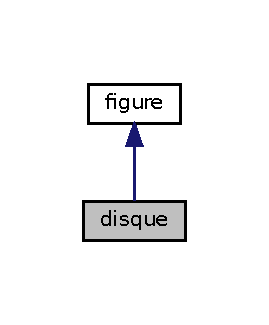
\includegraphics[width=129pt]{classdisque__inherit__graph}
\end{center}
\end{figure}


Collaboration diagram for disque\+:
\nopagebreak
\begin{figure}[H]
\begin{center}
\leavevmode
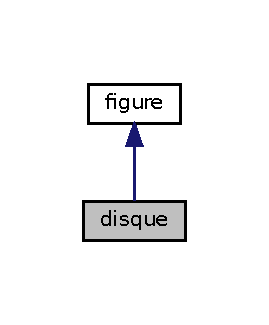
\includegraphics[width=129pt]{classdisque__coll__graph}
\end{center}
\end{figure}
\subsection*{Public Member Functions}
\begin{DoxyCompactItemize}
\item 
float \hyperlink{classdisque_ac26d8f8f1b149a7214f347ae9655410a}{Compute\+Perimeter} (float rayon)
\item 
float \hyperlink{classdisque_a144bd3137c6cd183eba6792a4553764b}{Compute\+Area} (float rayon)
\end{DoxyCompactItemize}


\subsection{Detailed Description}
calcul disque \{calcul air et perimetre du disque\} 

\subsection{Member Function Documentation}
\mbox{\Hypertarget{classdisque_a144bd3137c6cd183eba6792a4553764b}\label{classdisque_a144bd3137c6cd183eba6792a4553764b}} 
\index{disque@{disque}!Compute\+Area@{Compute\+Area}}
\index{Compute\+Area@{Compute\+Area}!disque@{disque}}
\subsubsection{\texorpdfstring{Compute\+Area()}{ComputeArea()}}
{\footnotesize\ttfamily float disque\+::\+Compute\+Area (\begin{DoxyParamCaption}\item[{float}]{rayon }\end{DoxyParamCaption})}


\begin{DoxyParams}{Parameters}
{\em rayon} & \{on calcul l\textquotesingle{}air avec le rayon et PI\} \\
\hline
\end{DoxyParams}
\begin{DoxyReturn}{Returns}

\end{DoxyReturn}
\mbox{\Hypertarget{classdisque_ac26d8f8f1b149a7214f347ae9655410a}\label{classdisque_ac26d8f8f1b149a7214f347ae9655410a}} 
\index{disque@{disque}!Compute\+Perimeter@{Compute\+Perimeter}}
\index{Compute\+Perimeter@{Compute\+Perimeter}!disque@{disque}}
\subsubsection{\texorpdfstring{Compute\+Perimeter()}{ComputePerimeter()}}
{\footnotesize\ttfamily float disque\+::\+Compute\+Perimeter (\begin{DoxyParamCaption}\item[{float}]{rayon }\end{DoxyParamCaption})}


\begin{DoxyParams}{Parameters}
{\em rayon} & \{on calcul le perimetre avec le rayon et PI\} \\
\hline
\end{DoxyParams}
\begin{DoxyReturn}{Returns}

\end{DoxyReturn}


The documentation for this class was generated from the following files\+:\begin{DoxyCompactItemize}
\item 
/home/aurelien/figure/src/\hyperlink{disque_8h}{disque.\+h}\item 
/home/aurelien/figure/src/disque.\+cpp\end{DoxyCompactItemize}

\hypertarget{classfigure}{}\section{figure Class Reference}
\label{classfigure}\index{figure@{figure}}


Inheritance diagram for figure\+:
\nopagebreak
\begin{figure}[H]
\begin{center}
\leavevmode
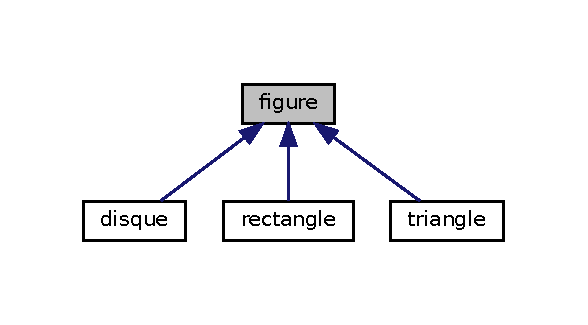
\includegraphics[width=282pt]{classfigure__inherit__graph}
\end{center}
\end{figure}
\subsection*{Public Member Functions}
\begin{DoxyCompactItemize}
\item 
virtual float \hyperlink{classfigure_ace592f5ccc0020afb1bee680b6806427}{Compute\+Perimeter} (int a)
\item 
virtual float \hyperlink{classfigure_a92c8c288812286ea31f401eb410146d9}{Compute\+Area} (int b)
\end{DoxyCompactItemize}


\subsection{Member Function Documentation}
\mbox{\Hypertarget{classfigure_a92c8c288812286ea31f401eb410146d9}\label{classfigure_a92c8c288812286ea31f401eb410146d9}} 
\index{figure@{figure}!Compute\+Area@{Compute\+Area}}
\index{Compute\+Area@{Compute\+Area}!figure@{figure}}
\subsubsection{\texorpdfstring{Compute\+Area()}{ComputeArea()}}
{\footnotesize\ttfamily float figure\+::\+Compute\+Area (\begin{DoxyParamCaption}\item[{int}]{b }\end{DoxyParamCaption})\hspace{0.3cm}{\ttfamily [virtual]}}


\begin{DoxyParams}{Parameters}
{\em b} & sera override \\
\hline
\end{DoxyParams}
\begin{DoxyReturn}{Returns}

\end{DoxyReturn}
\mbox{\Hypertarget{classfigure_ace592f5ccc0020afb1bee680b6806427}\label{classfigure_ace592f5ccc0020afb1bee680b6806427}} 
\index{figure@{figure}!Compute\+Perimeter@{Compute\+Perimeter}}
\index{Compute\+Perimeter@{Compute\+Perimeter}!figure@{figure}}
\subsubsection{\texorpdfstring{Compute\+Perimeter()}{ComputePerimeter()}}
{\footnotesize\ttfamily float figure\+::\+Compute\+Perimeter (\begin{DoxyParamCaption}\item[{int}]{a }\end{DoxyParamCaption})\hspace{0.3cm}{\ttfamily [virtual]}}


\begin{DoxyParams}{Parameters}
{\em a} & sera override \\
\hline
\end{DoxyParams}
\begin{DoxyReturn}{Returns}

\end{DoxyReturn}


The documentation for this class was generated from the following files\+:\begin{DoxyCompactItemize}
\item 
/home/aurelien/figure/src/\hyperlink{figure_8h}{figure.\+h}\item 
/home/aurelien/figure/src/figure.\+cpp\end{DoxyCompactItemize}

\hypertarget{classrectangle}{}\section{rectangle Class Reference}
\label{classrectangle}\index{rectangle@{rectangle}}


calcul rectangle \{calcul aire et perimetre\}  




{\ttfamily \#include $<$rectangle.\+h$>$}



Inheritance diagram for rectangle\+:
\nopagebreak
\begin{figure}[H]
\begin{center}
\leavevmode
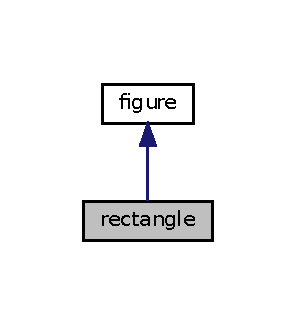
\includegraphics[width=142pt]{classrectangle__inherit__graph}
\end{center}
\end{figure}


Collaboration diagram for rectangle\+:
\nopagebreak
\begin{figure}[H]
\begin{center}
\leavevmode
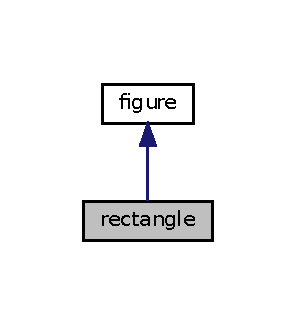
\includegraphics[width=142pt]{classrectangle__coll__graph}
\end{center}
\end{figure}
\subsection*{Public Member Functions}
\begin{DoxyCompactItemize}
\item 
float \hyperlink{classrectangle_ad9eb8dfdd783c528dd7a6011e0d89dcb}{Compute\+Perimeter} (float longueur, float largeur) override
\item 
float \hyperlink{classrectangle_a7dafa66d6ad61db0ba37c2b75ee50e4c}{Compute\+Area} (float longueur, float largeur) override
\end{DoxyCompactItemize}


\subsection{Detailed Description}
calcul rectangle \{calcul aire et perimetre\} 

\subsection{Member Function Documentation}
\mbox{\Hypertarget{classrectangle_a7dafa66d6ad61db0ba37c2b75ee50e4c}\label{classrectangle_a7dafa66d6ad61db0ba37c2b75ee50e4c}} 
\index{rectangle@{rectangle}!Compute\+Area@{Compute\+Area}}
\index{Compute\+Area@{Compute\+Area}!rectangle@{rectangle}}
\subsubsection{\texorpdfstring{Compute\+Area()}{ComputeArea()}}
{\footnotesize\ttfamily float rectangle\+::\+Compute\+Area (\begin{DoxyParamCaption}\item[{float}]{longueur,  }\item[{float}]{largeur }\end{DoxyParamCaption})\hspace{0.3cm}{\ttfamily [override]}}


\begin{DoxyParams}{Parameters}
{\em longueur} & \\
\hline
{\em largeur} & \{calcul largeur$\ast$longueur\} \\
\hline
\end{DoxyParams}
\begin{DoxyReturn}{Returns}

\end{DoxyReturn}
\mbox{\Hypertarget{classrectangle_ad9eb8dfdd783c528dd7a6011e0d89dcb}\label{classrectangle_ad9eb8dfdd783c528dd7a6011e0d89dcb}} 
\index{rectangle@{rectangle}!Compute\+Perimeter@{Compute\+Perimeter}}
\index{Compute\+Perimeter@{Compute\+Perimeter}!rectangle@{rectangle}}
\subsubsection{\texorpdfstring{Compute\+Perimeter()}{ComputePerimeter()}}
{\footnotesize\ttfamily float rectangle\+::\+Compute\+Perimeter (\begin{DoxyParamCaption}\item[{float}]{longueur,  }\item[{float}]{largeur }\end{DoxyParamCaption})\hspace{0.3cm}{\ttfamily [override]}}


\begin{DoxyParams}{Parameters}
{\em longueur} & valeur necessaire pour le calcul \\
\hline
{\em largeur} & valeur necessaire pour le calcul \{calcul (lageur+longuguer)$\ast$2\} \\
\hline
\end{DoxyParams}
\begin{DoxyReturn}{Returns}

\end{DoxyReturn}


The documentation for this class was generated from the following files\+:\begin{DoxyCompactItemize}
\item 
/home/aurelien/figure/src/\hyperlink{rectangle_8h}{rectangle.\+h}\item 
/home/aurelien/figure/src/rectangle.\+cpp\end{DoxyCompactItemize}

\hypertarget{classtriangle}{}\section{triangle Class Reference}
\label{classtriangle}\index{triangle@{triangle}}


calcul aire et perimetre d\textquotesingle{}un triangle  




{\ttfamily \#include $<$triangle.\+h$>$}



Inheritance diagram for triangle\+:
\nopagebreak
\begin{figure}[H]
\begin{center}
\leavevmode
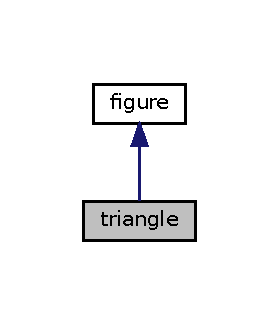
\includegraphics[width=134pt]{classtriangle__inherit__graph}
\end{center}
\end{figure}


Collaboration diagram for triangle\+:
\nopagebreak
\begin{figure}[H]
\begin{center}
\leavevmode
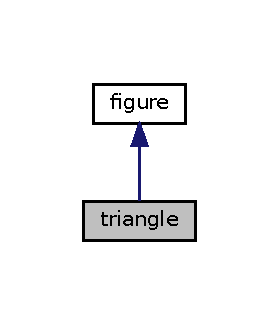
\includegraphics[width=134pt]{classtriangle__coll__graph}
\end{center}
\end{figure}
\subsection*{Public Member Functions}
\begin{DoxyCompactItemize}
\item 
float \hyperlink{classtriangle_a6bd90bcfd3a2e287577fa7654ee7c8c2}{Compute\+Perimeter} (float side1, float side2, float side3)
\item 
float \hyperlink{classtriangle_aff0e02134612db76cb599a0b85df566f}{Compute\+Area} (float base, float hauteur)
\end{DoxyCompactItemize}


\subsection{Detailed Description}
calcul aire et perimetre d\textquotesingle{}un triangle 

\subsection{Member Function Documentation}
\mbox{\Hypertarget{classtriangle_aff0e02134612db76cb599a0b85df566f}\label{classtriangle_aff0e02134612db76cb599a0b85df566f}} 
\index{triangle@{triangle}!Compute\+Area@{Compute\+Area}}
\index{Compute\+Area@{Compute\+Area}!triangle@{triangle}}
\subsubsection{\texorpdfstring{Compute\+Area()}{ComputeArea()}}
{\footnotesize\ttfamily float triangle\+::\+Compute\+Area (\begin{DoxyParamCaption}\item[{float}]{base,  }\item[{float}]{hauteur }\end{DoxyParamCaption})}


\begin{DoxyParams}{Parameters}
{\em base} & et hauteur. (Base $\ast$ hauteur)/2 \\
\hline
\end{DoxyParams}
\begin{DoxyReturn}{Returns}

\end{DoxyReturn}
\mbox{\Hypertarget{classtriangle_a6bd90bcfd3a2e287577fa7654ee7c8c2}\label{classtriangle_a6bd90bcfd3a2e287577fa7654ee7c8c2}} 
\index{triangle@{triangle}!Compute\+Perimeter@{Compute\+Perimeter}}
\index{Compute\+Perimeter@{Compute\+Perimeter}!triangle@{triangle}}
\subsubsection{\texorpdfstring{Compute\+Perimeter()}{ComputePerimeter()}}
{\footnotesize\ttfamily float triangle\+::\+Compute\+Perimeter (\begin{DoxyParamCaption}\item[{float}]{side1,  }\item[{float}]{side2,  }\item[{float}]{side3 }\end{DoxyParamCaption})}


\begin{DoxyParams}{Parameters}
{\em side1} & side2 side3 sont les valeurs des 3 cotes. On fait la somme pour trouver le perimetre \\
\hline
\end{DoxyParams}
\begin{DoxyReturn}{Returns}

\end{DoxyReturn}


The documentation for this class was generated from the following files\+:\begin{DoxyCompactItemize}
\item 
/home/aurelien/figure/src/\hyperlink{triangle_8h}{triangle.\+h}\item 
/home/aurelien/figure/src/triangle.\+cpp\end{DoxyCompactItemize}

\chapter{File Documentation}
\hypertarget{disque_8h}{}\section{/home/aurelien/figure/src/disque.h File Reference}
\label{disque_8h}\index{/home/aurelien/figure/src/disque.\+h@{/home/aurelien/figure/src/disque.\+h}}


calcul disque  


{\ttfamily \#include \char`\"{}figure.\+h\char`\"{}}\newline
Include dependency graph for disque.\+h\+:
\nopagebreak
\begin{figure}[H]
\begin{center}
\leavevmode
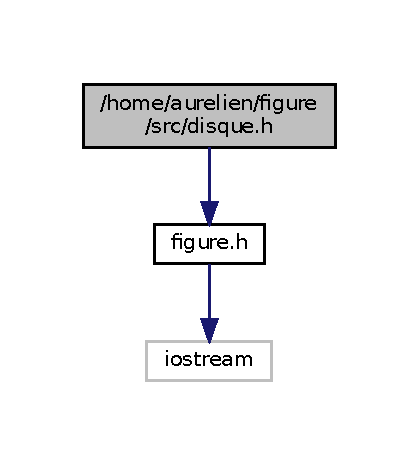
\includegraphics[width=201pt]{disque_8h__incl}
\end{center}
\end{figure}
\subsection*{Classes}
\begin{DoxyCompactItemize}
\item 
class \hyperlink{classdisque}{disque}
\begin{DoxyCompactList}\small\item\em calcul disque \{calcul air et perimetre du disque\} \end{DoxyCompactList}\end{DoxyCompactItemize}


\subsection{Detailed Description}
calcul disque 

\begin{DoxyAuthor}{Author}
Aurelien Guillemot 
\end{DoxyAuthor}
\begin{DoxyVersion}{Version}
1.\+0 
\end{DoxyVersion}

\hypertarget{figure_8h}{}\section{/home/aurelien/figure/src/figure.h File Reference}
\label{figure_8h}\index{/home/aurelien/figure/src/figure.\+h@{/home/aurelien/figure/src/figure.\+h}}


creation de l\textquotesingle{}objet figure  


{\ttfamily \#include $<$iostream$>$}\newline
Include dependency graph for figure.\+h\+:
\nopagebreak
\begin{figure}[H]
\begin{center}
\leavevmode
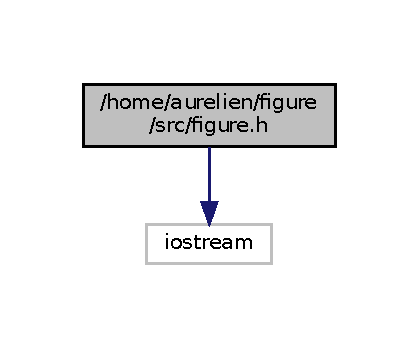
\includegraphics[width=201pt]{figure_8h__incl}
\end{center}
\end{figure}
This graph shows which files directly or indirectly include this file\+:
\nopagebreak
\begin{figure}[H]
\begin{center}
\leavevmode
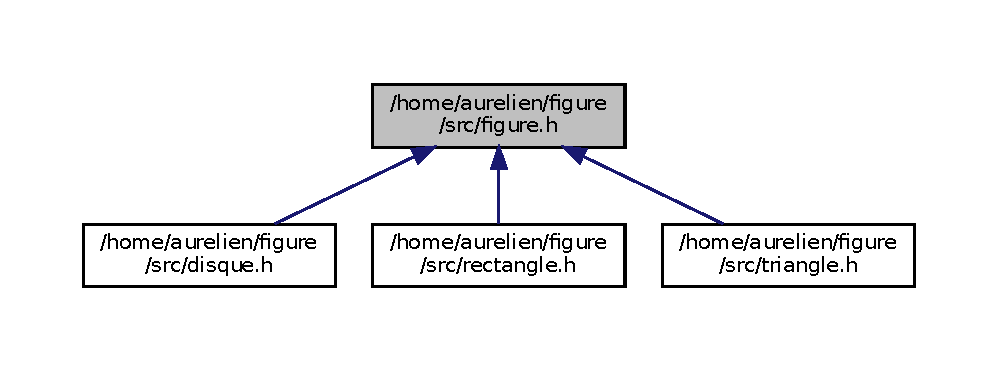
\includegraphics[width=350pt]{figure_8h__dep__incl}
\end{center}
\end{figure}
\subsection*{Classes}
\begin{DoxyCompactItemize}
\item 
class \hyperlink{classfigure}{figure}
\end{DoxyCompactItemize}


\subsection{Detailed Description}
creation de l\textquotesingle{}objet figure 

\begin{DoxyAuthor}{Author}
Aurelien Guillemot 
\end{DoxyAuthor}
\begin{DoxyVersion}{Version}
1.\+0 
\end{DoxyVersion}

\hypertarget{rectangle_8h}{}\section{/home/aurelien/figure/src/rectangle.h File Reference}
\label{rectangle_8h}\index{/home/aurelien/figure/src/rectangle.\+h@{/home/aurelien/figure/src/rectangle.\+h}}


calcul du perimetre et de l\textquotesingle{}aire du rectangle  


{\ttfamily \#include \char`\"{}figure.\+h\char`\"{}}\newline
Include dependency graph for rectangle.\+h\+:
\nopagebreak
\begin{figure}[H]
\begin{center}
\leavevmode
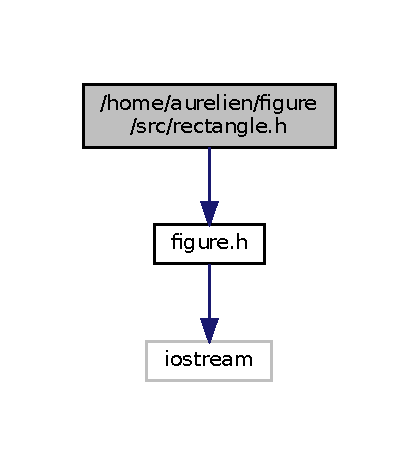
\includegraphics[width=201pt]{rectangle_8h__incl}
\end{center}
\end{figure}
\subsection*{Classes}
\begin{DoxyCompactItemize}
\item 
class \hyperlink{classrectangle}{rectangle}
\begin{DoxyCompactList}\small\item\em calcul rectangle \{calcul aire et perimetre\} \end{DoxyCompactList}\end{DoxyCompactItemize}


\subsection{Detailed Description}
calcul du perimetre et de l\textquotesingle{}aire du rectangle 

\begin{DoxyAuthor}{Author}
Aurelien Guillemot 
\end{DoxyAuthor}
\begin{DoxyVersion}{Version}
1.\+0 
\end{DoxyVersion}

\hypertarget{triangle_8h}{}\section{/home/aurelien/figure/src/triangle.h File Reference}
\label{triangle_8h}\index{/home/aurelien/figure/src/triangle.\+h@{/home/aurelien/figure/src/triangle.\+h}}


calcul perimetre et aire du triangle  


{\ttfamily \#include \char`\"{}figure.\+h\char`\"{}}\newline
Include dependency graph for triangle.\+h\+:
\nopagebreak
\begin{figure}[H]
\begin{center}
\leavevmode
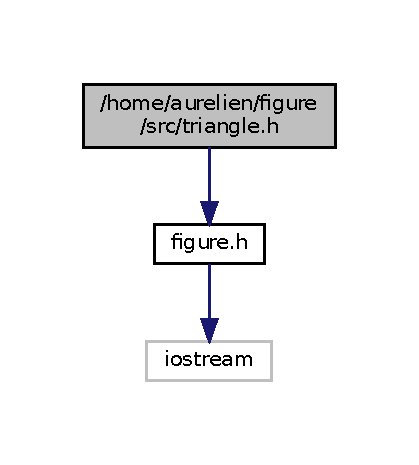
\includegraphics[width=201pt]{triangle_8h__incl}
\end{center}
\end{figure}
\subsection*{Classes}
\begin{DoxyCompactItemize}
\item 
class \hyperlink{classtriangle}{triangle}
\begin{DoxyCompactList}\small\item\em calcul aire et perimetre d\textquotesingle{}un triangle \end{DoxyCompactList}\end{DoxyCompactItemize}


\subsection{Detailed Description}
calcul perimetre et aire du triangle 

\begin{DoxyAuthor}{Author}
Aurelien Guillemot 
\end{DoxyAuthor}
\begin{DoxyVersion}{Version}
1.\+0 
\end{DoxyVersion}

%--- End generated contents ---

% Index
\backmatter
\newpage
\phantomsection
\clearemptydoublepage
\addcontentsline{toc}{chapter}{Index}
\printindex

\end{document}
